\section{Strange Phenomenon in Training with Gradient Descent}

We want to use gradient descent to solve the Poisson equations.
\begin{equation}
  \label{BilinearNodalBasis}
  \left\{
  \begin{array}{ll}
-u''=f, \quad on [0,1], \\
u(0)=u(1)=0.
\end{array}
\right.
\end{equation}

For a given $f=\pi^2sin(\pi x) $, we can calculate the true solution as $u=sin(\pi x)$. We also want to use gradient descent to calculate the numerical solution to compare the error.

We divide the unit interval into $n$ intervals equally and denote the boundary points as $x_i=\frac{i}{n+1}, i=0,1,...,n+1$. Then the interpolation of the true solution is $u_i=sin(\pi x_i)$. 

To compute the numerical solution, we first define 
\begin{equation}
J(v_h)=\frac12\int_0^1|v_h'|^2dx-\int_0^1fv_hdx.
\end{equation}
Let 
$$
\displaystyle v_h=\sum_{i=1}^n\nu_i\varphi_i,
$$
then 
$$
J(v_h)=I(\nu)=\frac12\nu^TA\ast\nu-b^T\nu
$$
and 
$$
\nabla I(\nu) =A\ast \nu -b.
$$
Here $A=(-1,2,-1)/h$
At the same time, let $\displaystyle u_h=\sum_{i=1}^n\mu_i\varphi_i,$
\begin{equation}\label{min}
\displaystyle u_h=\argmin_{v_h\in V_h} J(v_h)\Leftrightarrow \mu=\argmin_{\nu \in R^n} I(\nu)
\end{equation}

Therefore, we choose a random $u_0$, then in $i$-th iteration we update
\begin{equation}
u^i=u^{i-1}+\eta(b-A * u^{i-1}).
\end{equation}
We plot the graph of the $H_1$-norm of the error, $||u^i-u||$, vs the number of iteration $i$.

When we choose $k=4$ and $ \eta=\frac{h}{4},\frac{h}{8},\frac{h}{16},\frac{h}{32}$ respectively, the graphs of the $H_1$-norm of the error, $||u^i-u||$, vs the number of iteration $i$ are as follows.
\begin{figure}[!htbp]
	\begin{center}
		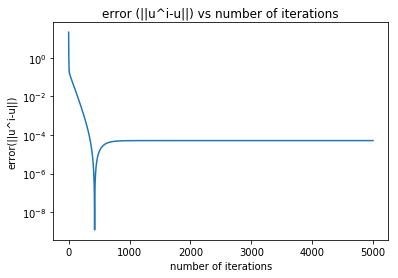
\includegraphics[width=0.45\textwidth]{./figures/h-4}  \quad 
		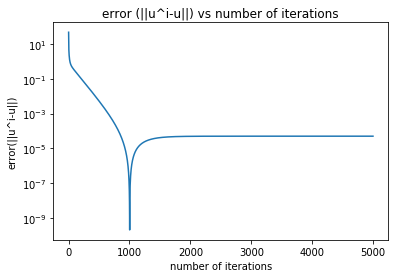
\includegraphics[width=0.45\textwidth]{./figures/h-8} \\ 
		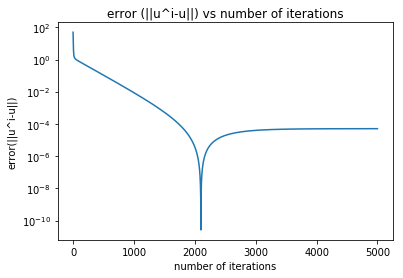
\includegraphics[width=0.45\textwidth]{./figures/h-16} \quad 
		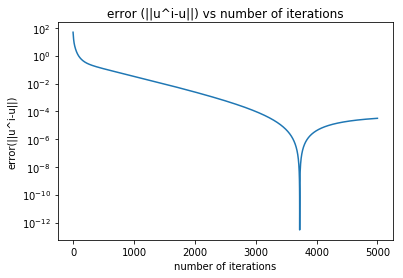
\includegraphics[width=0.45\textwidth]{./figures/h-32} 
	\end{center}
	\caption{error vs number of iteration for $\eta=\frac{h}{4},\frac{h}{8},\frac{h}{16},\frac{h}{32}$}
\end{figure}

There is a spike in  the graphs, where the error decreases very fast below $10^{-8}$ and then increase. Moreover, as $ \eta$ decreases, the number of iteration where the spike happens also increases. 

One explanation is that it's a special case when the interpolation of the true solution is a eigenvector of the matrix $A$. What we can do is to decrease the $ \eta$ accordingly to a very small value.